\begin{question}[class=A]{2}
  \label{question:true-false-a}
  True or False question version \GetVersionID. \\
  \begin{minipage}{0.85\textwidth}
    Statement...
  \end{minipage}%
  \begin{minipage}{0.15\textwidth}
    \begin{tasks}(1)
      \task[\choice] \ True
      \task[\correctchoice] \ False
    \end{tasks}
  \end{minipage}
\end{question}

\begin{question}[class=B]{2}
  \label{question:true-false-b}
  True or False question version \GetVersionID. \\
  \begin{minipage}{0.85\textwidth}
    Statement...
  \end{minipage}%
  \begin{minipage}{0.15\textwidth}
    \begin{tasks}(1)
      \task[\correctchoice] \ False
      \task[\choice] \ True
    \end{tasks}
  \end{minipage}
\end{question}

\noindent\rule{\textwidth}{1pt}

\begin{question}{3}
  \label{question:multiple-choice}
  Multiple Choice question. \\
  Statement...
  \begin{tasks}(4)
    \task[\choice] \ Choice 1
    \task[\correctchoice] \ Choice 2
    \task[\choice] \ Choice 3
    \task[\choice] \ Choice 4
  \end{tasks}
\end{question}

\noindent\rule{\textwidth}{1pt}

\begin{question}{3}
  \label{question:select-all}
  Select All question. \\
  Statement...
  \begin{tasks}(4)
    \task[\selectall] \ Choice 1
    \task[\correctselectall] \ Choice 2
    \task[\selectall] \ Choice 3
    \task[\selectall] \ Choice 4
  \end{tasks}
\end{question}

\noindent\rule{\textwidth}{1pt}

\begin{question}{3}
  \label{question:easy-problem}
  Easy problem with short work.
\end{question}
\begin{minipage}{0.75\textwidth}
  \begin{solution}
    Work.
  \end{solution}
\end{minipage}\hspace{\fill}%
\begin{minipage}{0.25\textwidth}
  \AnswerBox{Final Answer:}{0.5in}{Correct answer}
  \vspace{0.1in}
\end{minipage}

\noindent\rule{\textwidth}{1pt}

\begin{question}{6}
  \label{question:formula-problem}
  Problem that requires formula(s).
  \begin{tasks}(13)
    \task[\selectall] \ A
    \task[\selectall] \ B
    \task[\selectall] \ C
    \task[\selectall] \ D
    \task[\selectall] \ E
    \task[\selectall] \ F
    \task[\selectall] \ G
    \task[\correctselectall] \ H
    \task[\selectall] \ I
    \task[\selectall] \ J
    \task[\selectall] \ K
    \task[\selectall] \ L
    \task[\selectall] \ M
  \end{tasks}
\end{question}
\begin{minipage}{0.75\textwidth}
  \begin{solution}
    \[A^{-1} = \dfrac{1}{ad - bc}
      \begin{bmatrix}
        d & -b \\
        -c & a
      \end{bmatrix}
    \]
  \end{solution}
\end{minipage}\hspace{\fill}%
\begin{minipage}{0.25\textwidth}
  \vspace{0.5in}
  \AnswerBox{Final Answer:}{0.5in}{Correct answer}
  \vspace{0.1in}
\end{minipage}

\noindent\rule{\textwidth}{1pt}

\begin{question}{6}
  \label{question:setup-system}
  Setup variables and system of equations.\\[0.2in]
  \begin{minipage}{0.45\textwidth}
    \AnswerBox{Define Variables:}{0.5in}{Correct answer}
  \end{minipage}\hspace{\fill}%
  \begin{minipage}{0.45\textwidth}
    \AnswerBox{System of Equations:}{0.5in}{Correct answer}
  \end{minipage}
\end{question}

\noindent\rule{\textwidth}{1pt}

\newpage

\begin{question}{6}
  \label{question:graph-question}
  Problem with graph.\\
  \begin{minipage}{0.45\textwidth}
  \end{minipage}\hspace{\fill}%
  \begin{minipage}{0.5\textwidth}
    \begin{center}
      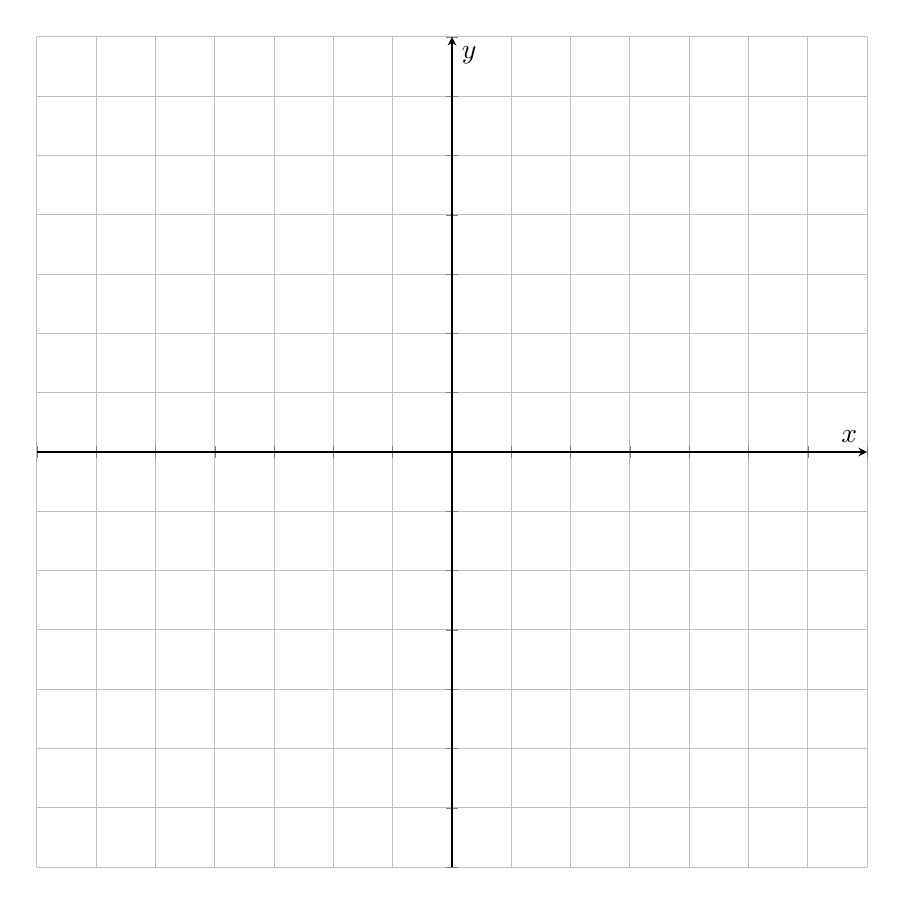
\begin{tikzpicture}
        \begin{axis}[%
          xmin = -7, xmax = 7, ymin = -7, ymax = 7,%
          xtick = {-8,...,8}, xticklabels = \empty,%
          ytick = {-8,...,8}, yticklabels = \empty,%
          axis x line = middle, axis y line = middle,%
          grid, xlabel = {\(x\)}, ylabel = {\(y\)},%
          width = \textwidth, height = \textwidth%
          ]
        \end{axis}
      \end{tikzpicture}
    \end{center}
  \end{minipage}
\end{question}

\noindent\rule{\textwidth}{1pt}
